\documentclass[11pt,a4paper]{article}
\usepackage[titletoc,toc,title]{appendix}
\usepackage{tikz}
\usetikzlibrary{matrix,chains,positioning,decorations.pathreplacing,arrows}
\usepackage[nottoc,notlot,notlof]{tocbibind}
% Modèle de rapport de stage et conseils de rédaction, mise en page...
% L. Bellon, avril 2010
\usepackage{listings}
% définition des marges du document
\setlength{\topmargin}{0cm}
\setlength{\headheight}{0.4cm}
\setlength{\headsep}{0.8cm}
\setlength{\footskip}{1cm}
\setlength{\textwidth}{17cm}
\setlength{\textheight}{25cm}
\setlength{\voffset}{-1.5cm}
\setlength{\hoffset}{-0.5cm}
\setlength{\oddsidemargin}{0cm}
\setlength{\evensidemargin}{0cm}
\usepackage{subfig}
% quelques package utiles
\usepackage{graphicx} % inclusion des figures
\usepackage{tikz}
\usepackage{amsmath} % collection de symboles mathématiques
\usepackage{amssymb} % collection de symboles mathématiques


\usepackage{pdfpages}
\makeatletter
\def\BState{\State\hskip-\ALG@thistlm}
\makeatother

%\usepackage[applemac]{inputenc}       % utilisation directe des caractères accentués sur mac
\usepackage[utf8]{inputenc}       % utilisation directe des caractères accentués sur pc
\usepackage[T1]{fontenc} % codage moderne des caractères sous Latex

\usepackage[francais]{babel}           % style français

\usepackage{tabularx} % gestion avancée des tableaux

\usepackage{psfrag} % remplacement du texte d'une figure ps par du texte latex
\usepackage{sistyle} % mise en forme des unités

\usepackage{eurosym} % symbole €
\def\€{\euro{}}

\usepackage{color} % gestion de différentes couleurs

\definecolor{linkcolor}{rgb}{0,0,0.6} % définition de la couleur des liens pdf
\usepackage[ pdftex,colorlinks=true,
pdfstartview=FitV,
linkcolor= linkcolor,
citecolor= linkcolor,
urlcolor= linkcolor,
hyperindex=true,
hyperfigures=false]
{hyperref} % fichiers pdf 'intelligents', avec des liens entre les références, etc.

\usepackage{fancyhdr} % entêtes et pieds de pages personnalisés

% définition de l'entête et du pied de page
\pagestyle{fancy}
\fancyhead[L]{\scriptsize \textsc{Dicotomix}}
\fancyhead[R]{\scriptsize \textsc{\'Equipe Dicotomix}}
\fancyfoot[C]{ \thepage}

% commande d'annulation du correcteur typographique du package [francais]{babel} qui force l'espace avant ':' (parfois utile pour la bibliographie)
\makeatletter
\@ifpackageloaded{babel}%
        {\newcommand{\nospace}[1]{{\NoAutoSpaceBeforeFDP{}#1}}}%  % !! double {{}} pour cantonner l'effet à l'argument #1 !!
        {\newcommand{\nospace}[1]{#1}}
\makeatother

% commande de déplacement d'un objet
\newcommand{\drawat}[3]{\makebox[0pt][l]{\raisebox{#2}{\hspace*{#1}#3}}}

\usepackage{amsthm}
\theoremstyle{plain}
\newtheorem{thm}{Théorème}[section] % reset theorem numbering for each chapter

\theoremstyle{definition}
\newtheorem{defn}[thm]{Définition} % definition numbers are dependent on theorem numbers

\begin{document}

% Pour faciliter la mise en forme de la page du titre, on supprime l'indentation automatique en début de paragraphe
\setlength{\parindent}{0pt}

% Pas d'en-tête ni de pied pour la première page
\thispagestyle{empty}


\includegraphics[height=2cm]{images/logoens.eps} \hfill \includegraphics[height=2cm]{images/logoucbl.eps} \hfill \includegraphics[height=2cm]{images/logounivlyon.eps}

\vspace{0.5cm}

\begin{tabularx}{\textwidth}{@{} l X l @{} }
{\sc Master d'informatique fondamentale} & & U.E Projet intégré\\
{\it École Normale Supérieure de Lyon} & & Équipe Dicotomix\ \\
{\it Université Claude Bernard Lyon I} & & \url{http://avalon.ens-lyon.fr/dicotomix/}
\end{tabularx}

\begin{center}


\vspace{1.5cm}

\rule[11pt]{5cm}{0.5pt}

\textbf{\huge Dicotomix}

\rule{5cm}{0.5pt}
\vspace{0.5cm}


\includegraphics[scale=0.7]{images/icon.eps}

\vspace{0.5cm}

T.Stérin, A.Martin, F.Lécuyer, \\ E.Hazard, P.Mangold, E.Kerinec, M.Guy, \\ R.Pellerin, N.Pinson, A.Słowik

\vspace{1.5cm}

\parbox{15cm}{\small
\textbf{Résumé} : \it TODOOOOOOOOOOO WTF Les réseaux de neurones récurrents sont des modèles aptes à apprendre et à générer des séquences temporelles. Ces réseaux se déclinent en plusieurs variantes dont les deux principales sont Vanilla et LSTM. À travers un exemple concret d'inférence grammaticale on constate la faiblesse des Vanilla à exploiter des dépendances temporelles longues. Sur la base de ces résultats expérimentaux on remet en cause l'importance de la raison la plus souvent invoquée dans la littérature pour expliquer cette faiblesse. On propose une autre explication que l'on conjuge avec l'introduction d'une mesure de la capacité de mémoire d'un modèle récurrent. On confronte cette mesure à la théorie des Echo States Networks qui aborde ces questions de mémoire différemment. Forts de ces expériences on applique les techniques décrites à la génération de musique à travers les chorals de Bach.

} %fin de la commande \parbox du résumé


\vspace{0.5cm}

\parbox{15cm}{
\textbf{Mots clefs} : \it un, deux, trois
} %fin de la commande \parbox des mots clefs

\vspace{1.5cm}

\parbox{15cm}{


\includegraphics[scale=0.24]{images/logo-hcl-plein_2995-bleu.jpg} \hfill

\includegraphics[scale=0.15]{images/ARS-Auvergne-Rhone-Alpes.jpg}
} %fin de la commande \parbox encadrant / laboratoire d'accueil

\vspace{0.5cm}
\vspace{0.5cm}
\end{center}

\vfill
\hfill \today
\newpage
% Pas d'entête ni de pied pour la page de sommaire
\thispagestyle{empty}
\section*{Remerciements}

\paragraph{}Tout d'abord, un grand merci à l'ENS de Lyon, au département informatique et à \href{http://graal.ens-lyon.fr/~ecaron/}{Eddy Caron} et \href{http://perso.ens-lyon.fr/issam.rais/}{Issam Raïs}, nos encadrants de projet. Merci pour la liberté dont nous avons joui dans l'organisation et la mise en \oe uvre de ce projet. Merci pour la confiance que vous nous avez témoignée tout au long de l'année.
Et enfin, merci de nous avoir donné l'occasion de réalisé un projet si prenant.

\paragraph{}
Nous tenons à remercier très sincèrement le professeur Jacques Luauté qui nous a très généreusement ouvert les portes de son service et toujours encouragés dans notre démarche.
Nous voulons aussi remercier le docteur Emilien Bernard pour l'expérience qu'il nous a apportée autour de la maladie de Charcot. Un grand merci à Perrine Seguin, interne 
du service, Melaine De Quelen et Manel Ben Romdhane, orthophonistes du service et aux externes qui ont organisé la réalisation de l'étude au quotidien. Enfin, un immemse merci
aux patients pour leur implication dans l'étude et pour tout ce qu'ils nous ont appris humainement.

\paragraph{}
Nous tenons particulièrement à remercier Maureen Clerc, Alexandra Corneyllie et Jérémie Mattout pour leur aide précieuse dans le domaine de la BCI.

\paragraph{}
Merci également à tous les linguistes intervenus dans le projet, Nicolas Laurent, Isabel Colón de Carvajal, Matthieu Quignard et Jean-Philippe Magué, qui ont contribué à nourrir notre réflexion et à permettre 
des améliorations à l'algorithme initial. Nous souhaitons aussi remercier très chaleureusement \href{http://www.charlie-lopez.com/}{Charlie Lopez} 
qui a réalisé tout le design graphique du logiciel. Enfin nous souhaitons remercier \href{http://thibaultsouquet.fr/}{Thibault Souquet} pour sa participation à la construction 
de l'architecture client-serveur du logiciel et à l'organisation visuelle de celui-ci.

\paragraph{}Enfin, un très grand merci à Odile Souquet, référente régionale pour la thématique médecine à l'Agence Régionale de Santé du Rhône-Alpes, qui nous a accompagnés tout au long de notre cheminement et a contribué à l'organisation de rencontres décisives pour le projet.

\newpage

\tableofcontents

\newpage
\section{Introduction}

\paragraph{} Le Locked-In Syndrome (\textbf{LIS}) est un état neurologique qui prive les patients de la quasi-totalité de leurs capacités motrices : ils ne peuvent ni bouger ni parler,
mais leurs capacités cognitives ne sont pas altérées \textit{a priori}. Les patients se retrouvent prisonniers de leur corps, d'où l'appellation de syndrome d'enfermement, parfois utilisée.
Cette maladie a notamment été présentée au grand public à travers \textit{Le Scaphandre et le Papillon}, mémoires retraçant le combat de Jean-Dominique Bauby pour communiquer. 
En effet, la motricité des yeux est généralement conservée et permet de mettre en place un code "Oui/Non" donnant un moyen élémentaire de communication.

\paragraph{} La communication, c'est cette problématique qui à l' du projet Dicotomix. La rencontre avec le monde hospitalier nous a fait comprendre que ce problème est plus général 
que le cadre strict du LIS car il concerne d'autres maladies, comme la maladie de Charcot ou sclérose latérale amyotrophique (\textbf{SLA}). Là où des études montrent ([ETUDE]) que communiquer est primordial pour le bien-être psychique des patients, d'autres insistent ([ETUDE 9 Chez Pauloss]) sur la pénibilité des méthodes traditionnelles. Ainsi, comment utiliser la technologie pour améliorer les moyens de communication de ces patients ? 

\paragraph{} Ce rapport a donc pour objectif de présenter les différentes solutions pensées par notre équipe pour répondre à ce problème. C'est grâce à l'intervention de nombreuses personnes du monde hospitalier que 
nous avons pu confronter nos "idées de laboratoire" aux besoins réels des patients et du monde médical. Cette confrontation a constamment guidé notre démarche et a conduit à notre réalisation principale, le logiciel Dicotomix.

\paragraph{} Enfin, nous avons eu la chance de pouvoir faire tester notre logiciel à un patient LIS et une patiente SLA, au cours d'une étude pilote menée avec les Hospices Civiles de Lyon.
Cet aboutissement, très intense humainement, a redessiné une nouvelle fois les contours du projet. De sa genèse à l'étude pilote, c'est l'aventure humaine et scientifique du projet Dicotomix.


\section{Genèse du projet}

L'idée initiale du projet est née à la suite d'une conférence de Maureen Clerc à l'ENS de Lyon. Elle est une des spécialistes français de l'Interface Cerveau Machine (\textbf{BCI} pour Brain Computer Interface).
Les interfaces cerveaux machines constituent l'ensemble des techniques qui permettent d'interagir avec un ordinateur à l'aide de l'activité cérébrale. Sa conférence était orientée autour de l'électroencéphalographie (\textbf{EEG}), qui étudie les activités électriques du cerveau grâce à un casque d'électrodes posées sur le scalp (Figure \ref{eeg}). Il s'agissait d'une introduction aux techniques permettant d'exploiter informatiquement ces signaux EEG.

\begin{figure}[ht]
\centering
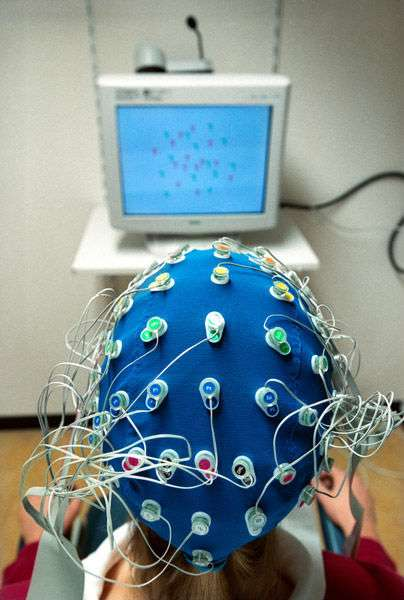
\includegraphics[scale=0.3]{images/electroencephalogramme.jpg}
\caption{Casque d'EEG et interface cerveau machine}
\label{eeg}
\end{figure}

\paragraph{} L'idée était alors la suivante : utiliser les signaux EEG pour permettre au patient de répondre à des questions fermées que pose la machine.
Autrement dit, le but était d'associer à certains signaux cérébraux que le patient choisit d'émettre la réponse "Oui" et aux autres la réponse "Non". 
C'est sur cette idée, de répondre à des questions, qu'est construite l'application \href{http://fr.akinator.com/}{Akinator}. Elle devine, et souvent très rapidement, 
un personnage auquel on pense. Ainsi, sous réserve d'élargir le procédé à n'importe quel type d'objet, cette méthode pouvait servir d'alternative aux méthodes traditionnelles de communication.

\paragraph{} Ces méthodes traditionnelles, que nous avons regroupées dans notre étude comparative (voir Annexe B), reposent toutes sur le même principe : énumérer les
lettres de l'alphabet au patient et attendre qu'il dise oui au moment où l'on annonce la sienne. Lettre par lettre, les mots sont ainsi épelés. Tout l'enjeu de notre démarche est de penser une solution moins frustrante [ETUDE 9 Chez Pauloss] que l'épellation. Le système de réponse à des questions, type Akinator, était notre premier candidat.

\paragraph{} Ainsi, deux grands axes de réflexion se sont dégagés très tôt dans notre travail :
\begin{itemize}
\item \textbf{L'interface}, c'est à dire le moyen physique de dire "Oui" ou "Non". Ici, les signaux EEG contre le mouvement des yeux.
\item \textbf{La méthode} pour exprimer un mot une fois que l'on est capable de dire "Oui" ou "Non" -- peu importe le moyen. Ici, la méthode Akinator contre 
les méthodes traditionnelles d'épellation.
\end{itemize}

\paragraph{} Les deux prochaines parties détaillent nos travaux dans les deux branches et comment, au fil de nos interactions avec le monde hospitalier, nous avons transformé nos approches pour en arriver à Dicotomix.

\subsection{Interface cerveau machine}
\subsubsection{Casque EEG}
La première partie de notre travail en BCI a consisté à se renseigner autour du matériel dont on pouvait bénéficier pour réaliser nos expériences EEG. Deux catégories se sont alors dessinées:
\begin{itemize}
    \item Le matériel d'hôpital, très performant -- très bonne résolution des signaux -- donc très onéreux ($\sim$20k \euro{}) et difficile d'accès à l'hôpital (besoin d'accréditations).
    \item Le matériel pour particuliers. Il existe des modèles de BCI à des fins expérimentales dont la résolution
    est faible mais suffisante pour des premiers résultats. Le budget est sensiblement différent ($\sim$600 \euro{}).
\end{itemize}

\paragraph{} Nous nous sommes donc orientés vers les solutions pour particuliers où deux possibilités se présentent à nouveau :
\begin{itemize}
    \item Du matériel propriétaire, édité par la société Emotiv. Le code associé au matériel (SDK) est protégé et peu malléable.
    \item Du matériel libre édité par l'organisation \href{http://openbci.com/}{OpenBCI} à la philosophie entièrement open software et open hardware (le casque est 3D imprimable).
\end{itemize}
C'est sous les conseils de Maureen Clerc que nous nous sommes orientés vers le matériel OpenBCI dont elle nous avait attesté la qualité.

\paragraph{} C'est grâce à Alexandra Corneyllie et Jérémie Mattout, ingénieure de recherche et chercheur spécialistes en BCI, que nous avons pu avoir accès au casque \texttt{Ultracortex Mark IV} d'OpenBCI (Figure \ref{openbci}) qu'ils nous ont prêté pendant toute la durée de notre projet.

\begin{figure}[h!]
\centering
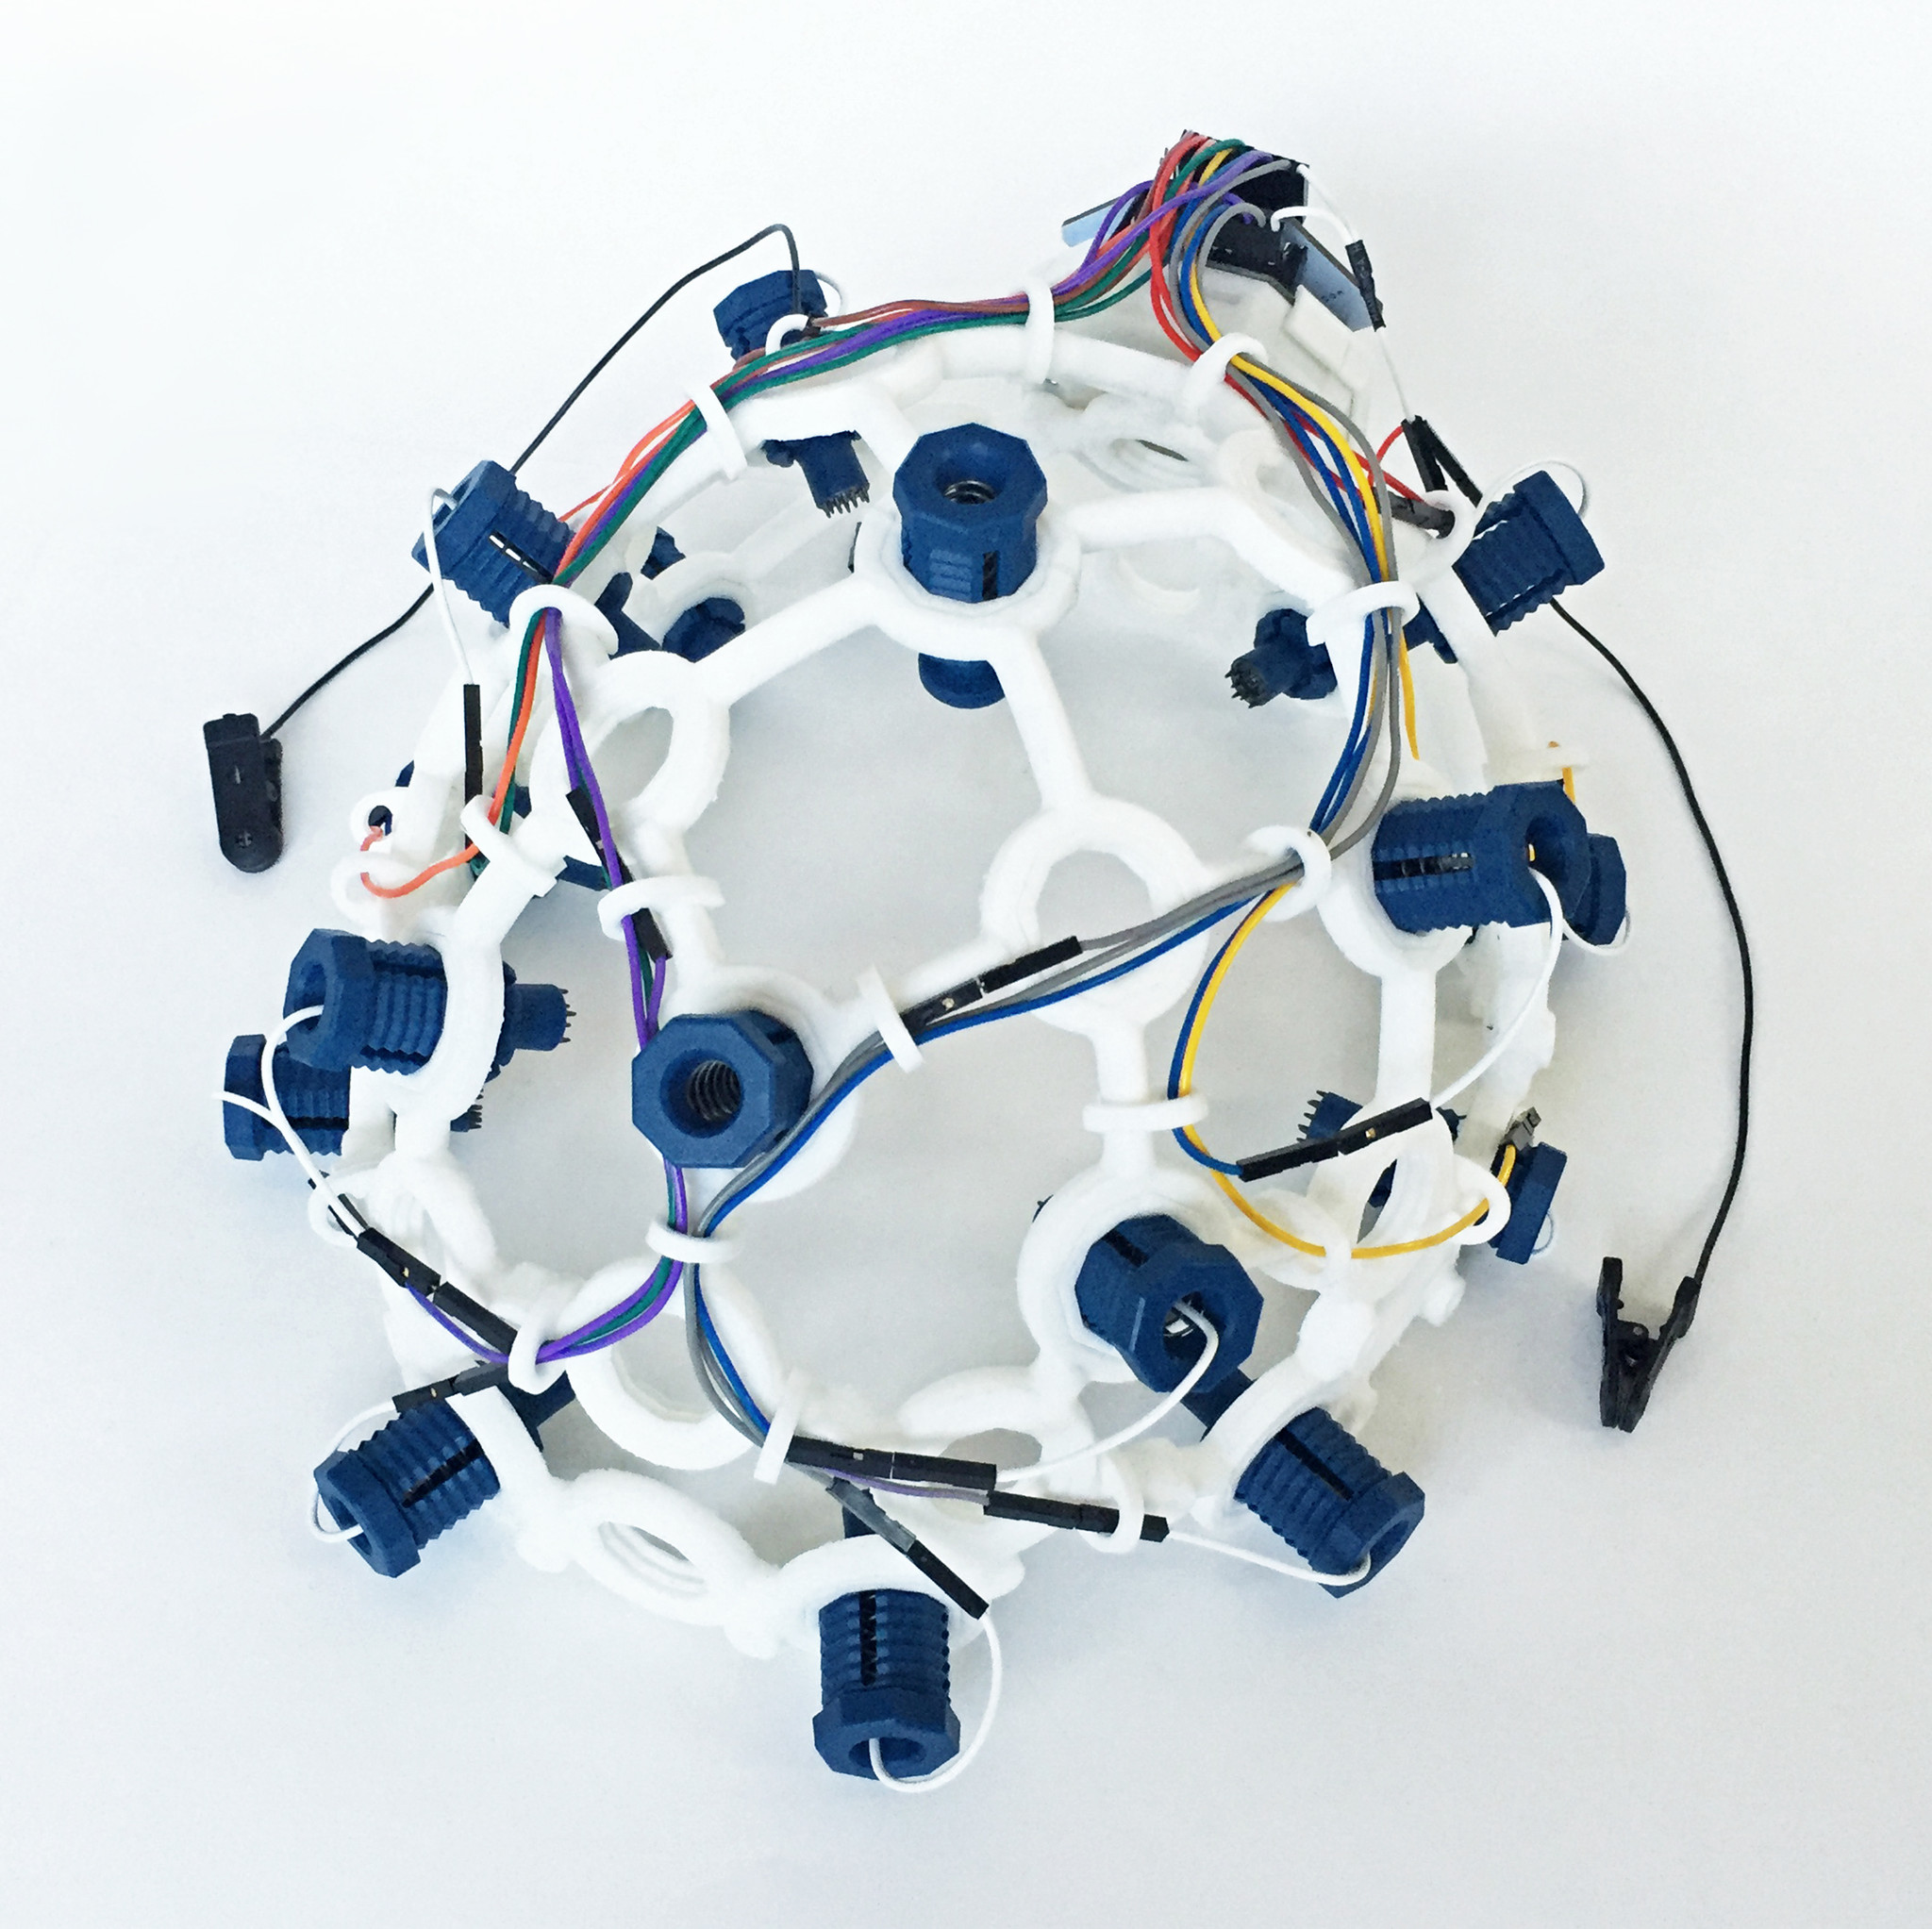
\includegraphics[scale=0.05]{images/OpenBCI.jpg}
\caption{Ultracortex Mark IV, casque EEG OpenBCI}
\label{openbci}
\end{figure}

\paragraph{} Nous avions pour ambition d'être capables de détecter un signal binaire avec le casque EEG, c'est-à-dire de concevoir une situation qui permet au patient
d'indiquer par son activité cérébrale un "Oui" ou un "Non". Nous avons envisagés deux paradigmes EEG parmi les plus simples de la discipline : les ondes alpha et 
le SSVEP. 

\subsubsection{Paradigme Alpha}

\paragraph{} Lorsqu'on fermer les yeux ou qu'on se relaxe, le cerveau produit avec une intensité plus élevée que la moyenne des composantes à 10Hz que l'on retrouve en position O1 du système 10-20 (Figure \ref{dix}).
Ces composantes sont appelées ondes Alpha [REF NECESSAIRE]. Il s'agit donc de repérer ces pics de fréquence à 10Hz et de les associer à une réponse, par
exemple "Oui". La Figure \ref{eeghack} montre les résultats en temps fréquence issus d'un blog d'expert [REF EEG HACKER] contre les meilleures données que nous avions pu générer en Figure \ref{ouralph}, suite à un enregistrement des ondes cérébrales d'une personne de l'équipe avec le casque EEG.

\begin{figure}[h!]
\centering
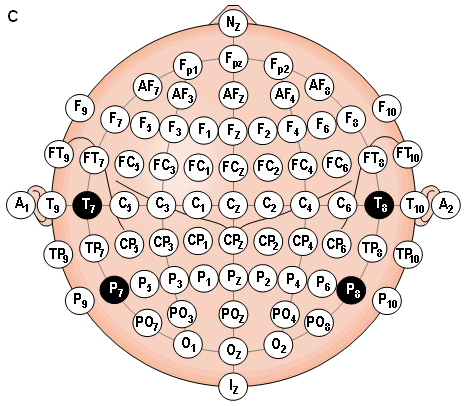
\includegraphics[scale=0.4]{images/1020.png}
\caption{Système 10-20, norme de placement des électrodes pour les casques EEG}
\label{dix}
\end{figure}

\paragraph{} On voit que les siennes sont très discriminées. Les notres sont plus hasardeuses : on en voit seulement autour de 110s alors qu'elles auraient dû apparaître sur toute la période temporelle. Notre expérimentation avec les ondes alpha n'a pas été concluante. Pour expliquer cet échec, plusieurs possibilités ont été suggérées :
\begin{itemize}
	\item l'acquisition des ondes dépend de nombreux paramètres comme la position des électrodes, le placement du casque, l'immobilité des fils et câbles ; il est donc probable que notre configuration n'ait pas été optimale.
	\item l'émission des $\alpha$ est sujet-dépendante : certaines personnes en produisent moins que d'autres. Comme nous avons principalement testé sur une même personne, l'absence d'ondes $\alpha$ peut être inhérente au sujet.
	\item les ondes alpha sont bruitées par d'autres sources électromagnétiques et par l'activité cérébrale annexe du sujet. Un manque de concentration, l'appréhension ou l'excitation dues à l'expérience, peuvent avoir nui à la relaxation et donc à l'émission $\alpha$.
\end{itemize}

\begin{figure}[h!]
\centering
\caption{Ondes alpha : résultats d'expert}
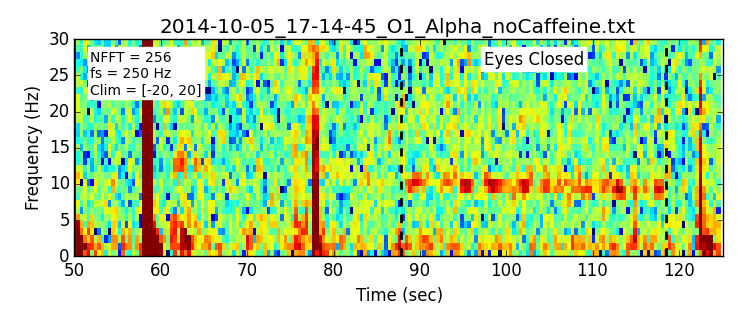
\includegraphics[scale=0.5]{images/eeghackerAlpha.png}
\label{eeghack}%
\end{figure}
\begin{figure}[h!]
\centering
\caption{Ondes alpha : nos résultats}
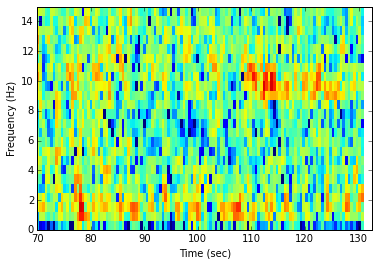
\includegraphics[scale=0.5]{images/ourAlpha.png}
\label{ouralph}%
\end{figure}

\subsubsection{Paradigme SSVEP}

\paragraph{} Le paradigme SSVEP repose sur le phénomène de potentiel évoqué [REFERENCE]. Si l'on présente à un sujet une image qui clignote à une certaine fréquence (entre 5 et 10Hz dans nos expériences) on retrouve 
des pics à cette fréquence dans l'activité du cortex visuel (électrodes O1 et O2 sur la Figure \ref{dix}). L'idée est donc de proposer deux sources lumineuses qui clignotent à deux fréquences différentes sur l'écran (une pour Oui et une pour Non), et de repérer le choix du patient en fonction de celle sur laquelle il porte son attention. Le même blog d'expert [EEG HACKER] réussit à contrôler un robot à l'aide de ce paradigme.
Malgré tous nos essais nous n'avons rien obtenu de concluant. Cela est très certainement dû aux raisons suivantes:

\begin{itemize}
\item Des problèmes d'acquisitions : des physiciens de l'ENS, spécialistes de l'EEG, ont remis en cause la qualité de nos signaux. Un mauvais placement du casque ou un paramétrage approximatif du logiciel d'acquisition peuvent en être à l'origine.
\item Un manque de contrôle sur la fréquence exacte à laquelle la vignette clignote. Jérémie Mattout, spécialiste de l'EEG, nous avait suggéré un protocole
plus fin pour se débarasser de ce biais à l'aide d'électro-photodiodes. Nous n'avons pas réussi à aboutir non plus.
\end{itemize}

\subsubsection{Conclusions}

\paragraph{} Les difficultés que nous rencontrions avec l'EEG devaient nous inciter à persévérer. Cependant, le professeur Luauté, que nous avons rencontré à mi-parcours (janvier), nous a très vite mis en garde sur la faisabilité de notre démarche. En effet, alors même que nous n'arrivions pas à obtenir des résultats satisfaisants sur des sujets sains, les équipes de recherches spécialistes du domaine butaient à faire fonctionner ces paradigmes chez les patients cérébrolésés [VOIR LES TROIS DOSSIER REFERENCES/HARD]. Il nous a invités à nous concentrer en priorité sur la méthode que nous voulions mettre en \oe uvre pour traiter ces signaux Oui/Non, arguant que nous pourrions la tester avec le code Oui/Non occulaire que beaucoup de ses patients utilisent. 

\paragraph{} Nous avons donc laissé de côté nos investigations autour de l'interface BCI pour nous concentrer sur la méthode de communication. Toutefois nous avons appris beaucoup de choses pendant cette phase du projet et nous nous sommes familiarisés avec un ensemble de techniques et de protocole expérimentaux qui nous étaient inconnus. De cette investigation pluridisciplinaire, nous tirons une idée plus claire de la réalité et des enjeux des interfaces cerveau-machine.

\subsection{Akinator}

TODO\\

Blabla: au début Akinator. Trop compliqué car besoin que des gens l'entrainent [METTRE LA REF SUR LE FONCTIONNEMENT AKINATOR (voir tout debut du projet)]. 
COmment simplifier Akinator ? DICHOTOMIE. Dire que l'idée embale Luauté.


\section{La solution Dicotomix}
 
\subsection{L'algorithme Dicotomix}
%Parler d'abord de dicotomix sur l'ensemble du dictionnaire avec astuces de randomisation pour cadavre et les autres petits tricks.\\
\paragraph{} Pour une entrée de type Oui/Non, le plus efficace est d'optimiser chaque question en l'utilisant pour diviser par deux le nombre de possibilités,  d'où l'idée d'une simple dichotomie.
Cependant, opérer ainsi sur l'ensemble des mots du dictionnaire n'est pas suffisant, puisque cela consiste à séparer à chaque étape en deux parties contenant le même nombre de mots, tandis que nous voulons deux parties de même probabilité. 
C'est pourquoi nous procédons par dichotomie pondérée par des fréquences pour chaque mot, ce qui revient à opérer sur un segment ou chaque mot à une longueur proportionnelle à sa fréquence (figure \ref{algo}).

\begin{figure}[h!]
\centering
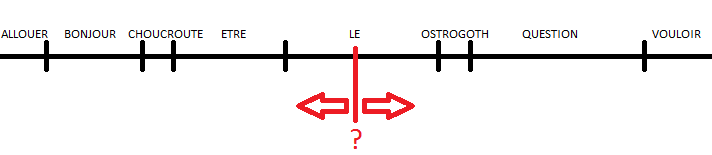
\includegraphics[scale=0.6]{schema_algo.png}
\caption{Schéma du fonctionnement de l'algorithme}
\label{algo}
\end{figure}

Pour déterminer la fréquence de chaque mot, nous avons utilisé une base de données donnant les fréquences des mots de la langue française en se basant sur des livres et des films. Nous avons ensuite ajouté quelques astuces en réponse à différents problèmes.\\
Un premier problème, d'apparence anodine, est le déterminisme de cet algorithme, qui a plusieurs effets négatifs : le côté répétitif pour l'utilisateur, le fait de tomber sur un mot très improbable situé juste à côté d'un mot souvent utilisé, ou encore l'apparition fréquente d'un mot désagréable (une version de l'algorithme menait très régulièrement au mot "cadavre"). Nous avons réglé ce problème en ajoutant un léger facteur aléatoire lorsque l'on coupe un segment en deux, pour ne pas tomber systématiquement sur le même mot.\\
Après cette modification, il a fallu mettre en place une mémorisation du chemin pour pouvoir revenir sur ses pas, puisque cette opération n'était plus déterminisée par la position actuelle.\\
TODO \\
Parler ensuite du spelling Mode et de la prédiction de lettre grace aux 5-grams (remercier linguistes Quignard et Magué pour l'idée blabla).\\
Dire qu'on pourrait faire du ngrams sur les mots pour prediction de mots.\\
Mentionner les techniques à l'état de l'art dans le domaine LSTM et réseaux de neurones récurrents. \\
Insister que Dicotomix en bénéficierai bcp. \\ 
DIRE LE MOT INTELLIGENCE ARTIFICIELLE \\
Dire que Luauté était emballé.  \\
P.e: reprendre les schémas de la pres

\subsection{Le logiciel}
TODO\\
Archi client serveur \\
JS \\
BLABLA c'est portable (testé sur MAC Linux et Windows pour de vrai) \\
plz: dire ce qu'à "fait" Souquet. + charlie Lopez. \\
Des ptites captures d'écran du futur. \\

\section{L'étude pilote}

\subsection{Le cadre}

Le professeur Jacques Luauté nous a accueilli au Service de Rééducation Post Réanimation (\textbf{SRPR}) de l'hôpital neurologique 
Pierre Wertheimer (Vinatier). C'est dans ce service que nous avons rencontré un patient atteint de LIS afin de pouvoir lui faire tester Dicotomix.
Perrine Seguin, interne du service, les équipes d'orthophonistes ainsi que les externes en médecine nous ont accompagné tout au long de 
la réalisation de l'étude. \\

Le docteur Émilien Bernard nous a mis en relation avec une patiente atteinte de SLA. Nous sommes allés la rencontrer à domicile.
Ainsi notre étude pilote a reposé sur des tests réalisés chez un patient LIS et une patiente SLA.

\subsection{La méthodologie}

La méthodologie de l'étude a été pensée avec l'équipe du professeur Luauté et est résumée Figure \ref{etude}. Delphine Maucort-Boulch spécialiste de méthodologie 
dans le cadre de ce type d'étude nous a aidé à finaliser le protocole.

\begin{figure}[h!]
\centering
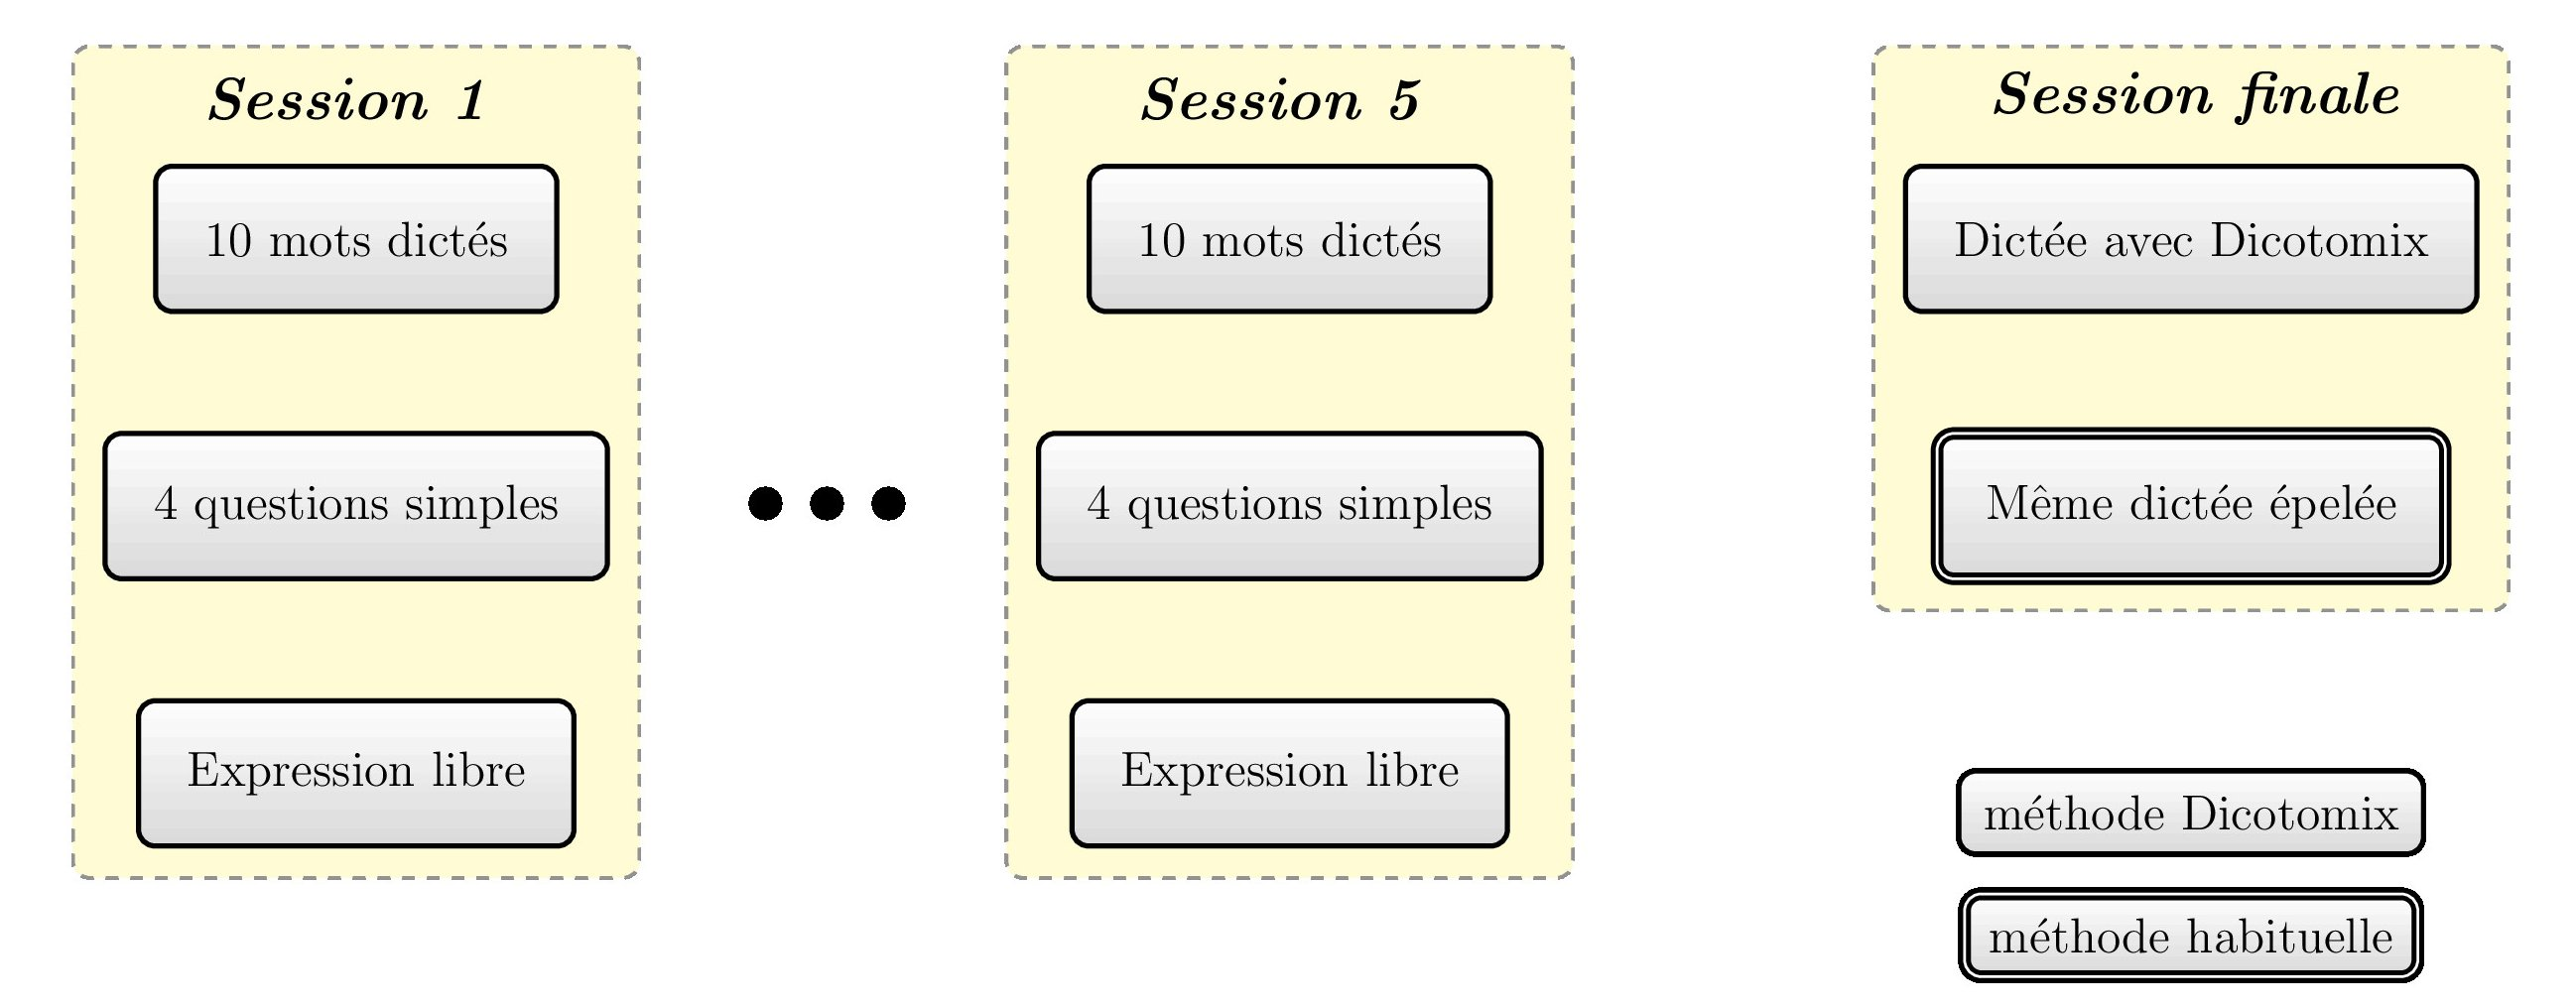
\includegraphics[scale=0.2]{images/schemaEtudePilote.jpg}
\caption{Méthodologie de l'étude pilote}
\label{etude}
\end{figure}

Il s'agissait d'abord d'entraîner le patient à utiliser le logiciel au cours de 5 sessions d'entraînement -- une par jour. Chaque sessions 
consistant à lui demander de trouver 10 mots dictés avec la méthode; puis de répondre à quatre questions simples ("Quelle est votre couleur préférée ?"); et 
enfin de le laisser s'exprimer librement avec l'outil s'il le souhaitait. \\
Ensuite, pour la session finale ou session d'évaluation, on dicte le même texte deux fois et le patient doit l'écrire la première fois avec Dicotomix puis avec
sa méthode habituelle. La même limite de temps est imposée pour les deux dictées et il s'agit donc de voir jusqu'où le patient a pu aller avec chacune des 
deux méthodes.


\subsection{La réalisation}

Nous avons commencé par tester le protocole avec le patient LIS. Entièrement paralysé, son code "Oui" / "Non" consistait à lever les yeux vers le ciel 
pour "Non" et les fermer pour "Oui". \\
La réalité a bien sûr eu raison de notre méthodologie. Très éprouvante en pratique notre méthodologie a été simplifiée à l'extrême. On ne demandais jamais plus de 5 mots 
au patient. Le mode Dicotomix est vite abandonné face à des difficultés trop grandes pour le patient -- il ne fallait surtout pas le décourager. Nous nous sommes donc limité
au mode épellation. Les externes du service ont grandement contribué à la réalisation de l'étude en visitant le patient quotidiennement et lui proposant des jeux, type pendu, 
pour rendre les sessions d'entraînement ludiques. 

\paragraph{}Ce patient a perdu la volonté de s'exprimer avec le personnel médical, il s'agissait de voir si notre méthode pouvait la
 lui rendre. Cela n'a pas été le cas car le patient n'a jamais voulu réaliser une "expression libre". Cependant nous avons pris conscience que le plus important pour lui, au delà de la 
 méthode pour communiquer, était la présence humaine. Ainsi à la quesion "voulez vous que l'on s'en aille ?", que l'on posait par peur de l'avoir trop fatigué, il répondait toujours "non". \\
 Le coût cognitif de notre méthode, que nous redoutions tant s'est fait sentir le jour de l'évaluation. En effet le patient est allé deux fois plus vite avec sa 
 méthode traditionnelle qu'avec Dicotomix. Même si elle sont moins rapides en théorie, les méthodes traditionnelles se défendent bien car l'énumération du tableau de lettres
 va très vite. La première idée que donne cette expérience, dans la veine de la prédiction de lettres du mode épellation, serait de dynamiser les tableaux de lettres traditionnels
 pour qu'ils se recomposent à chaque lettre épelée pour favoriser les prochaines lettres les plus probables. 

\paragraph{}Nous avons pu rencontrer une patiente SLA pour tester le même protocole à domicile. Possédant encore la mobilité de ses mains nous avons pu communiquer par mail autour de la méthode.
Cette patiente, qui a écrit plusieurs livres alors qu'elle était déjà malade, a vu en notre méthode plus quelque chose de ludique que de manifestement pratique. Aussi, malheureusement, un problème 
d'encodage des accents sur son PC (Windows) l'a empêché de mener à terme ses essais avec le logiciel. La préoccupation majeure de cette patiente était plus celle de l'interface, eye-tracker, head-tracker que
celle de la méthode. Encore un élément que le contact avec la réalité nous a permis de réaliser.

\section{Conclusion}

Le projet Dicotomix est avant tout une histoire de rencontres. Rencontres avec des disciplines différentes comme la BCI ou la linguistique, avec des univers différents comme le monde hospitalier. 
Mais surtout rencontres avec des personnes, toutes passionnées, qui ont donné sens à ce que nous voulions faire. 
\paragraph{}Cette expérience nous a initié au défi que représente le fait de vouloir réaliser une idée. Défi car, 
c'est à mesure que l'on se rapproche de sa concrétisation, de son passage à la réalité, que celle-ci se re-modèle et change de forme. Elle change de forme sous la contrainte de cette réalité
qui en est l'unique juge. Exactement suivant ce principe, alors que les résultats de l'étude pilote sont mitigés, ils nous ont dévoilé de nombreux moyens d'améliorer la technique. À commencer par en utiliser
uniquement la composante prédictive afin de construire un tableau de lettre interactif.
\paragraph{}Persuadés que pour être poursuivi dans des conditions sérieuses ce projet nécessiterait un investissement à plein temps de notre part et face à l'éparpillement qui attend notre équipe avec l'entrée 
en M2, nous avons pris la décision de le laisser reposer pour le moment. Tous nous abordons des parcours différents et nos regards croisés pourront enrichir, dans le futur, notre rapport 
à la problématique principale de Dicotomix. Pour l'heure, elle nous laisse forts de tout ce que l'on peut apprendre en allant à la rencontre des autres.

\newpage
\appendix
\section{Intervenants extérieurs et chronologie détaillée}
\paragraph{} La Figure \ref{grapheIntervenants} montre les principaux intervenants extérieurs qui ont participé à l'élaboration ou à la mise en place du projet. Y sont également représentés les différents liens entre ces personnes et leurs catégories de profession. Ce graphe permet de comprendre d'un coup d'\oe il l'organisation des participants ; une étude chronologique permet cependant une meilleure appréhension des interactions que nous avons eues avec ces personnes, et de leur influence sur le projet.
\begin{figure}[h!]
\centering 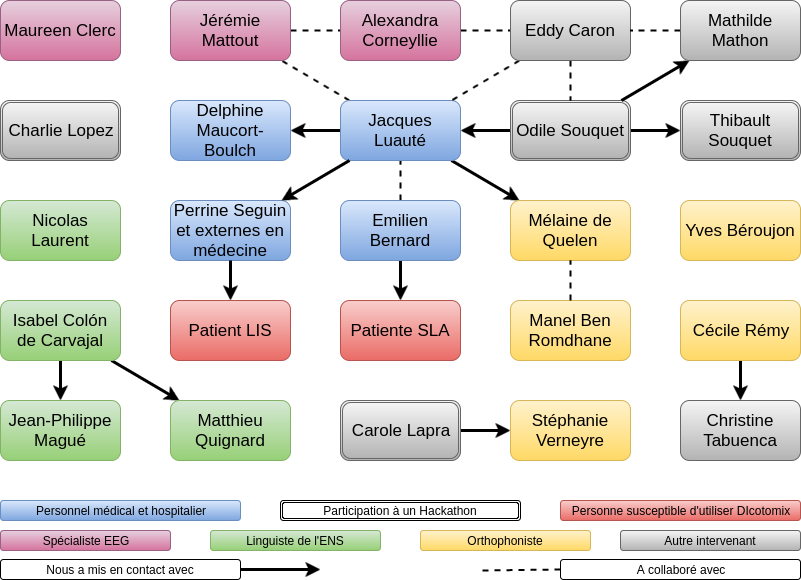
\includegraphics[width=16.4cm]{images/grapheIntervenants.png}
\caption{Graphe des intervenants}
\label{grapheIntervenants}
\end{figure}

\textbf{Octobre : } Rendez vous téléphonique avec \textbf{Maureen Clerc}, spécialiste de la BCI à l'INRIA Grenoble. Prise de connaissance de ses travaux autour du paradigme \textbf{P300} et des \textbf{P300-spellers}. Son équipe publiera bientôt ses résultats autour de leur système d'épellation P300 présenté comme le plus performant au monde. Comme vous le verrez dans la synthèse nous n'utilisons pas ce paradigme mais pourrons donc \textbf{comparer} notre méthode à celle-ci.\\

\textbf{9 novembre : } Rendez vous avec Yves Béroujon et son équipe de la fondation OVE. Ces orthophonistes travaillent au contact de jeunes malentendants. Première confrontation avec les \textbf{systèmes d'expression à base d'images}, piste un temps considérée pour notre projet.  \textbf{Problème :} le caractère trop peu formalisé de ces méthodes qui les rend difficiles à implémenter de manière générale. \\

\textbf{10 novembre : } rendez-vous téléphonique avec \textbf{Carole Lapra}, docteur qui nous mettra en relation avec des professionnels de santé spécialisés dans le domaine qui nous intéresse. \\

\textbf{18 novembre : } rendez vous avec \textbf{Stéphanie Verneyre} par l'intermédiaire de Carole Lapra, du service de neurologie de l'hôpital neurologique Pierre Wertheimer. Spécialiste de l'aphasie, Mme.Verneyre nous a aidé à \textbf{cibler} les pathologies pour lesquelles notre méthode pourrait être efficace. Nous découvrons à cette occasion la maladie de Charcot (SLA). \\

\textbf{18-20 novembre : } participation au Hackathon "Hacking Health". Nous rencontrons de nombreux professionnels de santé notamment \textbf{Odile Souquet} médecin à l'ARS (Agence régionale de Santé) qui n'a eu cesse par la suite de nous accompagner de manière très personnalisée. Nous lui devons parmi les rencontres les plus déterminantes pour notre projet. \\

\textbf{19 novembre : } rencontre avec \textbf{Alexandra Corneyllie} du CNRS qui nous a prêté le système de BCI que nous utilisons. Madame Corneyllie est l'une de nos interlocuteurs principaux sur la partie BCI du projet. \\

\textbf{22 décembre : } rencontre téléphonique avec \textbf{Jérémie Mattout}, spécialiste de la BCI et de ses applications à la médecine au CNRS, dans l'équipe d'Alexandre Corneyllie. À la suite de cette discussion \textbf{nous adoptons définitivement le paradigme SSVEP} (au lieu de P300) pour notre interface. Sous ses conseils, nous empruntons un générateur basse-fréquence et une led au laboratoire de physique. Ce dispositif nous permet de contrôler précisément notre système oscillant et pallie les difficultés que nous avons rencontrées avec la BCI. \\

\textbf{3 janvier : } rencontre avec le Professeur \textbf{Jacques Luauté}, via Odile Souquet, chef du service de rééducation neurologique à l'hôpital Henry Gabrielle. M. Luauté nous explique que faire marcher la BCI chez les sujets handicapés est un défi non encore résolu par les chercheurs spécialistes comme M. Mattout. Cependant le Professeur se montre très enthousiaste quand à notre méthode dichotomique d'énumération du dictionnaire. Il nous propose de la tester dès février étant donné que tous ses patients disposent déjà d'interfaces personnalisées pour exprimer 'oui' ou 'non'. Nous nous focalisons donc sur cette partie du projet pour fournir une solution à tester lors de nos rencontres de février. Cette rencontre souligne l'importance de se mettre en relation avec des linguistes. \\

\textbf{6 janvier : } réunion avec \textbf{Charlie Lopez}, rencontrée au Hackathon, graphiste qui a réalisé l'interface utilisateur de notre programme. \\

\textbf{17 janvier : } rencontre avec \textbf{Nicolas Laurent}, professeur de grammaire à l'ENS. Discussion autour des aspects linguistiques de notre projet. Il nous suggère de nous mettre en relation avec le laboratoire de linguistique informatique \textbf{ICAR} de l'ENS de Lyon. \\

\textbf{6 février : } rencontre avec \textbf{Cécile Remy}, via Odile Souquet, spécialiste des \textbf{SLA} qu'elle soigne à domicile. \\

\textbf{10 février : } nouveau rendez vous avec le professeur Luauté pour présenter l'avancement de nos travaux et mettre en place l'étude pilote. \\

\textbf{3-4 mars : } paraticipation au Hackathon "Hive" de l'école centrale Lyon. \\

\textbf{10 mars : } rencontre avec Mathilde Mathon autour de la métropole de Lyon. \\

\textbf{16 mars : } rencontre avec la linguiste Isabel Colon de Carvajal qui nous éclaire sur les base de données linguistiques d'interactions orales -- notamment dans le domaine de la médecine. \\

\textbf{17 mars : } nouvelle réunion de travail avec le professeur Luauté et son équipe. Nous rencontrons notamment le docteur Émilien Bernard grâce à qui nous avons pu aller à la rencontre d'une patiente SLA. \\

\textbf{24 mars : } réunion avec le professeur Luauté et Delphine Maucort-Boulch autour de la méthodologie de l'étude pilote. \\

\textbf{31 mars : } rencontre avec les linguistes spécialistes de Traitement Automatique des Langues, Matthieu Quignard et Jean-Philippe Magué. Ils nous exposent les différentes techniques que l'on peut implémenter dans le cadre de la prédiction de mots. À commencer par les n-grams.\\

\textbf{5-23 avril : } étude pilote. \\
    

\section{Étude comparative de la solution Dicotomix}
\paragraph{} Voir ci-après.
\section{Tutoriel d'utilisation de Dicotomix}
\paragraph{} Voir ci-dessous.

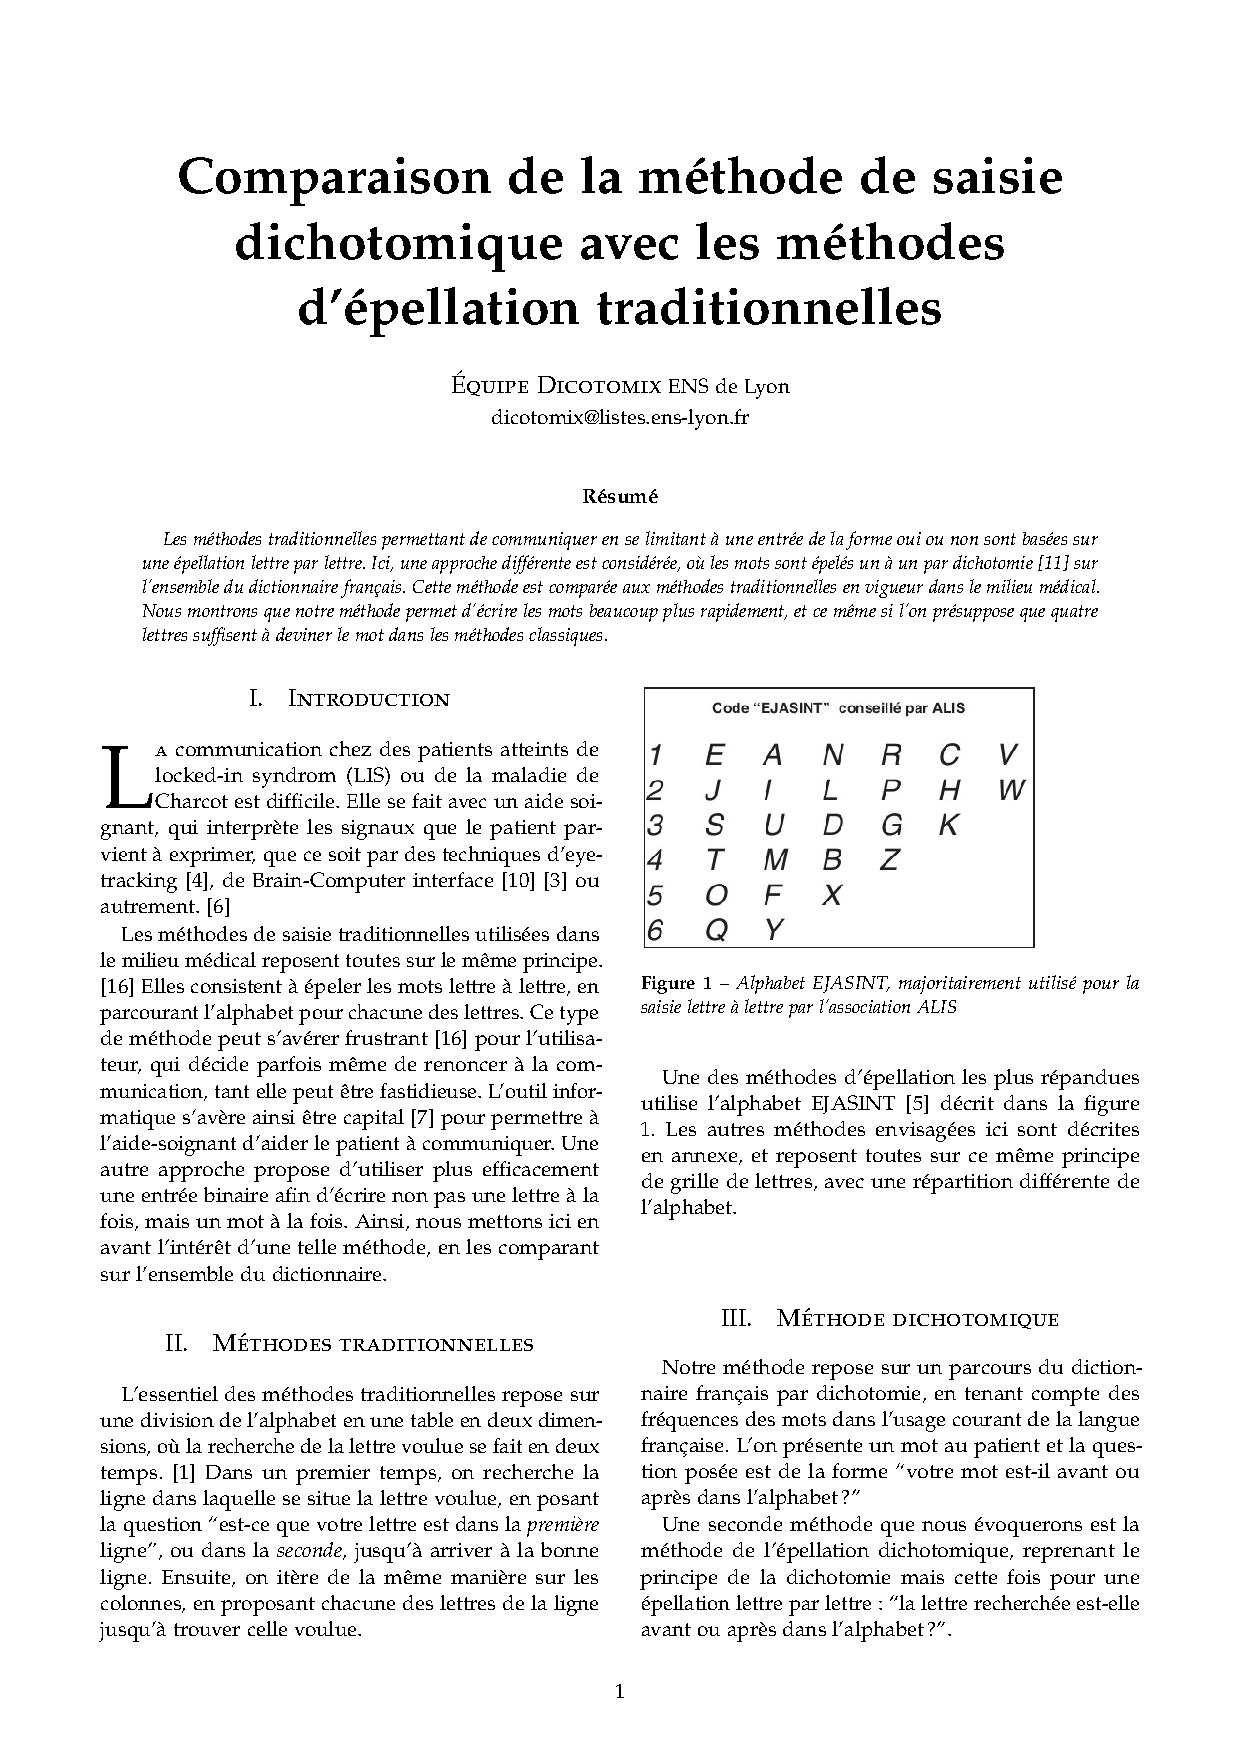
\includepdf[pages=-]{comparison.pdf}
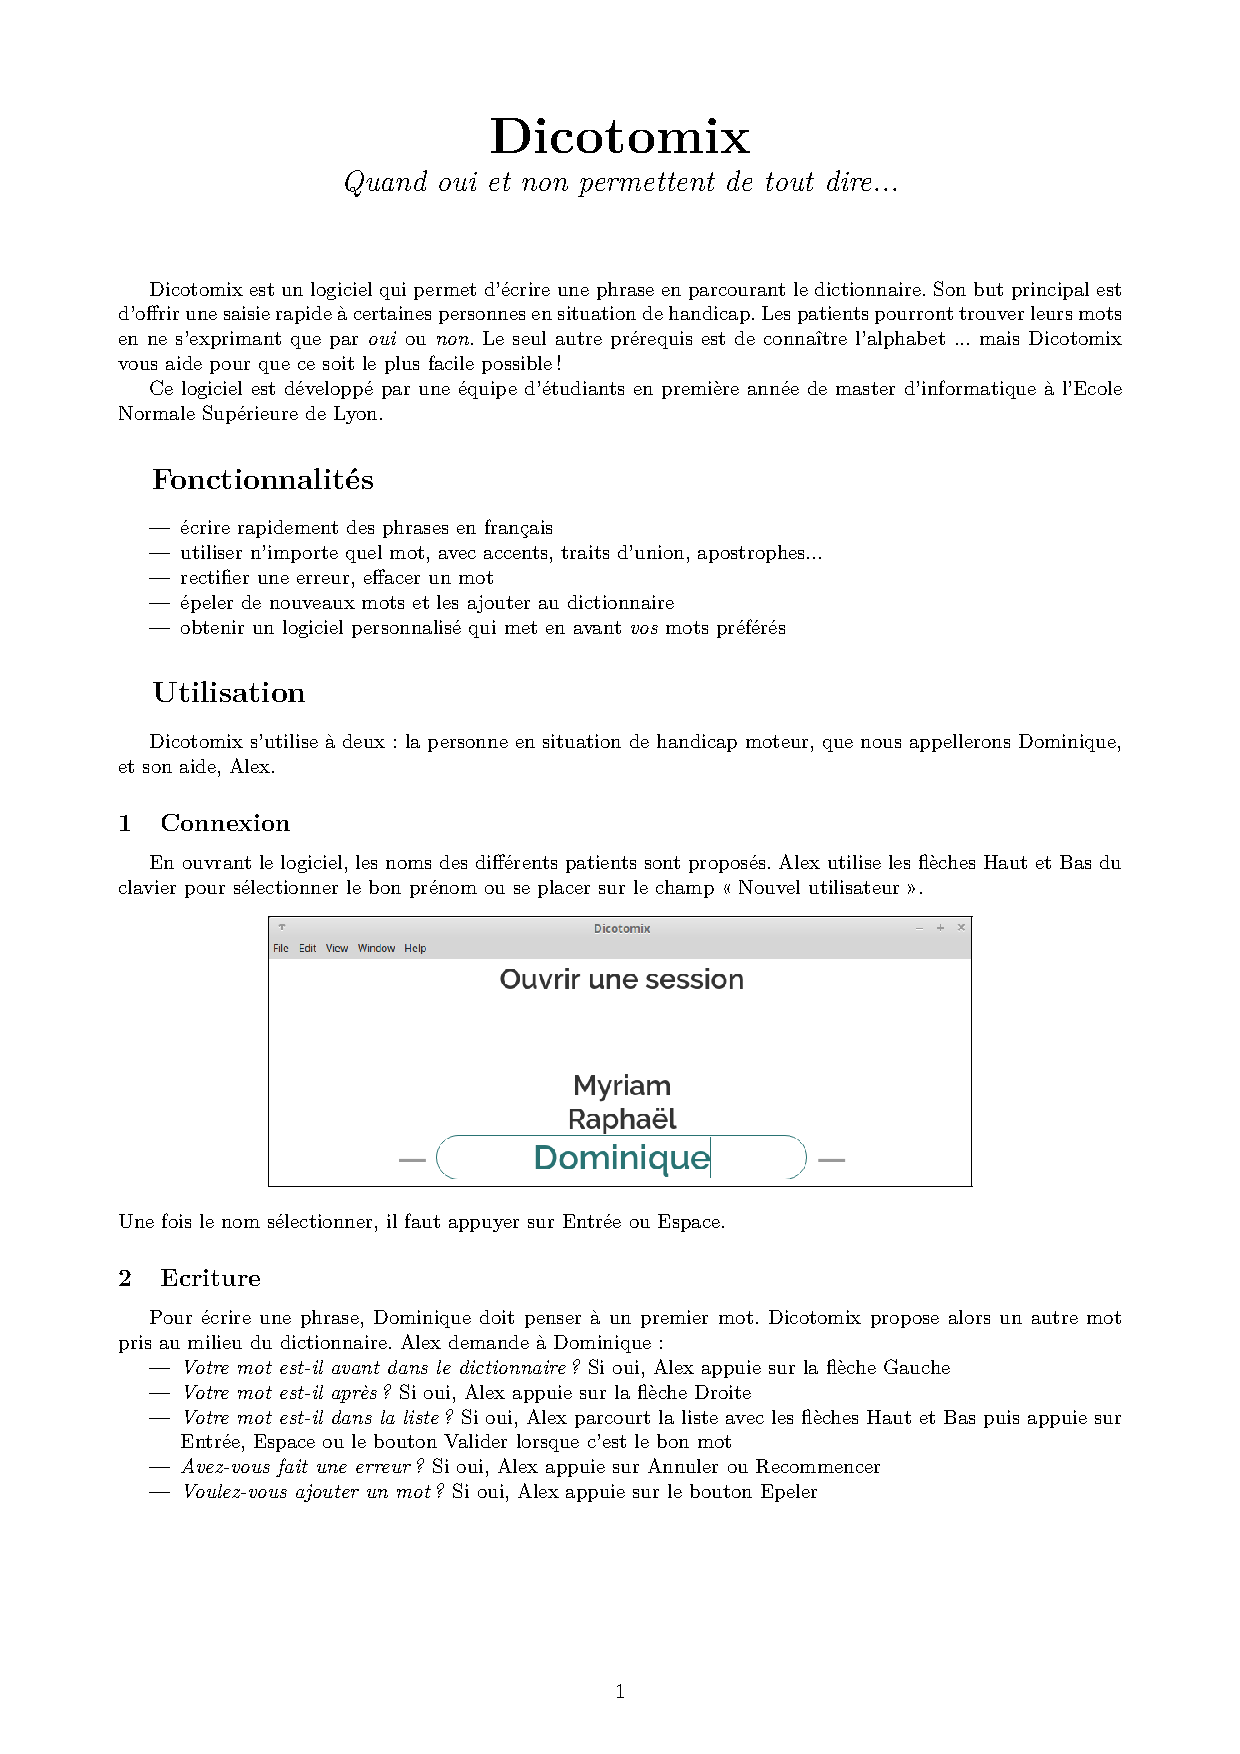
\includepdf[pages=-]{tutoriel.pdf}
\end{document}